\documentclass[]{report}
\usepackage{geometry}
\usepackage[utf8]{inputenc}
\usepackage{amsmath}
\usepackage{amsfonts}
\usepackage{amssymb}
\usepackage[pdftex]{graphicx}
\usepackage[space]{grffile}
\usepackage{epstopdf}
\usepackage{epsfig}
\usepackage{bmpsize}
\graphicspath{{./images/}}
\usepackage[export]{adjustbox}
\usepackage{wrapfig}
\usepackage{appendix}
\usepackage{listings}
\usepackage{hyperref}
\hypersetup{
	colorlinks=true,
	allcolors=blue,
	pdfborderstyle={/S/U/W 1}
}
\usepackage{hypcap}

% Add semantic reference commands
\newcommand*{\figref}[1]{%
	\hyperref[{#1}]{Figure~\ref*{#1}}%
}%
\newcommand*{\chapref}[1]{%
	\hyperref[{#1}]{\nameref{#1},~Kapital~\ref*{#1}}%
}%
\newcommand*{\secref}[1]{%
	\hyperref[{#1}]{\nameref{#1},~Sektion~\ref*{#1}}%
}%

\title{THM Benutzerhandbuch \\Untis \& THM Organizer}
\author{James Antrim}

\begin{document}
\maketitle

\newpage
\thispagestyle{empty}
\section*{}

\newpage
\tableofcontents
\thispagestyle{empty}

\newpage
\setcounter{page}{1}


\chapter{Allgemeine Untis-Bedienungshinweise}

Guten Tag! Ich habe ein kleines Handbuch erstellt, welches den Ein- bzw. Umstieg zur Untis 2015 erleichtern soll.\\
\\
Untis 2015 bietet viele neue Funktionen, welche die Arbeit mit Untis erheblich vereinfachen. Außerdem bietet die Software nun viele Einstellungsmöglichkeiten um die Darstellung bequemer und persönlicher zu gestalten. Das folgende Kapitel wird Ihnen dabei behilflich sein, Untis an Ihre persönlichen Bedürfnisse anzupassen und den Umgang mit der Vielfalt an Ansichten zu erleichtern.\\
\\

\section{Ribbon-Oberfläche und neue Menüführung}

Sehr auffällig bei Untis 2015 ist der Umstieg auf die, für Benutzer von Microsoft-Produkten vertraute, Ribbon-Oberfläche. 

\begin{figure}[h]
	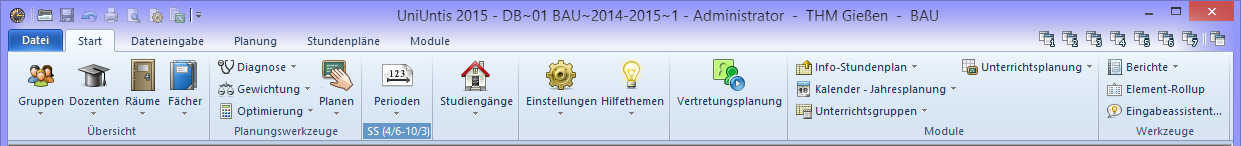
\includegraphics[width=1\textwidth]{ribbon-menu}
	\vspace{-15pt}
	\caption{Ribbon Oberfläche}
	\label{fig:ribbon}
\end{figure}

\noindent
Dies führt zu einem übersichtlicherem Hauptmenü mit wenigen Menüpunkten. Außerdem sind viele der Untermenüpunkte sofort sichtbar, was die Navigation deutlich erleichtert. Auch viele der Ressourcen-bezogenen Menüpunkte wurden unter den entsprechenden Ressourcen zusammengefasst. Beispielsweise sind die Ansichten für Gruppenverwaltung, Unterrichte (Gruppen-bezogen), und sämtliche Gruppenpläne jetzt Untermenüpunkte von Gruppen.  

\subsection{Menü Personalisierung}

Neu ist auch die Möglichkeit, die Menüleiste nach Belieben anzupassen. Unter Anderem die in der Schnellzugriff-Leiste angebotenen Ansichten, die deren Positionierung, und die Anzeige der Ribbon-Oberfläche.\\

\begin{wrapfigure}{r}{0.4\textwidth}
	\vspace{-4pt}
	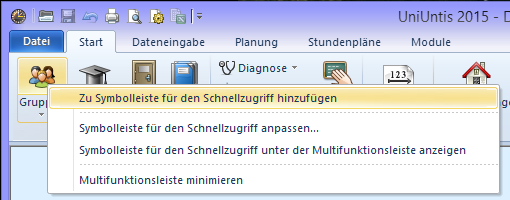
\includegraphics[width=.38\textwidth]{context-menu}
	\vspace{-5pt}
	\caption{Kontext Menü}
	\label{fig:context-menu}
	\vspace{50pt}
	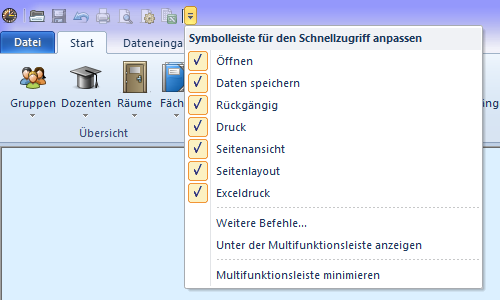
\includegraphics[width=.38\textwidth]{remove-quick-access-item}
	\vspace{-5pt}
	\caption{Vordefinierte Symbole\newline Entfernen}
	\label{fig:remove-quick-access-item}
	\vspace{4pt}
\end{wrapfigure}

\noindent
Um der Schnellzugriff-Leiste eine Ansicht hinzuzufügen, öffnet man das Kontext-Menü (Rechtsklick) und klickt auf den ersten Eintrag 'Zu Symbolleiste für den Schnellzugriff hinzufügen'. Hiermit kann man häufig verwendete Ansichten schneller, bzw. ohne die Menüführung zu verwenden, öffnen.\\
\\
Es gibt zwei Methoden, Elemente aus der Schnellzugriff-Leiste zu entfernen. Wenn das Symbol nicht standardmäßig angeboten wird (falls Sie das Symbol selbst hinzugefügt haben), verwendet man ebenfalls das Kontext Menü zum entfernen der Elemente. Nach einem Rechtsklick auf ein solches Symbol erscheint als erste Option 'Aus Symbolleiste für den Schnellzugriff entfernen', welche das Symbol von der Leiste entfernt.\\
\\
Um vordefinierte Symbole wie 'Öffnen' oder 'Datei Speichern' zu entfernen, klickt man auf das Symbol (kleiner Pfeil nach unten) direkt rechts von der Leiste. Dies öffnet ein neues Kontext-Menü, welches die vordefinierten dargestellten Symbole mit einem Häkchen davor anzeigt. Um die unerwünschten Symbole aus der Liste zu entfernen, muss nun das entsprechende Häkchen entfernt werden.\\
\\
Da die Ribbon-Oberfläche die Arbeitsfläche verringert, bietet die Software über das Kontext-Menü die Möglichkeit, diese zu minimieren. Dies hat als Folge, dass die Ribbon-Oberfläche nur sichtbar wird wenn man einen der Hauptmenüpunkte anklickt. Das Standardverhalten kann man von überall in der Menüleiste, durch das Entfernen der entsprechenden Häkchen vom Kontext-Menü, wiederherstellen.\\
\\
Letztlich kann man auch die Schnellzugriff-Leiste unterhalb der Ribbon-Oberfläche darstellen lassen, in dem man im Kontext-Menü auf den dritten Punkt 'Symbolleiste für den Schnellzugriff unter der Multifunktionsleiste anzeigen' klickt. So eingestellt, kann man die Leiste auf ihre Ursprungsposition bringen, in dem man nochmal auf den dritten Punkt des Kontext-Menüs klickt.\\
\\
Weiter fortgeschrittene Personalisierungseinstellungen erreicht man unter der Verwendung der Schaltfläche Personalisierung, Sektion \secref{sec:advanced-quick-access}.

\newpage

\subsection{Standard Fenstergruppen}

\begin{wrapfigure}{r}{0.4\textwidth}
	\vspace{-14pt}
	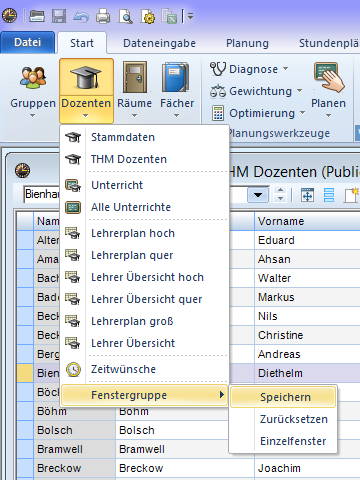
\includegraphics[width=.38\textwidth]{default-window-grouping}
	\vspace{-5pt}
	\caption{Felder der Ansicht Icon}
	\label{fig:default-window-grouping}
	\vspace{-10pt}
\end{wrapfigure}

Eine weitere Neuheit, verbunden mit der Zusammenführung der Ressourcen-Ansichten, sind die Standard-Fenstergruppen. Wenn man auf die großen Symbole der Hauptressourcen klickt, öffnet sich erstmal eine vordefinierte Gruppierung von Ansichten, welche mit dieser Ressource zusammenhängen. Durch ein Klick auf das Tür-Symbol, zum Beispiel, werden alle bereits geöffneten Ansichten geschlossen und die Ansichten Stammdaten, Zeitwünsche, Raumplan Hoch, und Unterricht geöffnet.\\
\\
Obwohl die voreingestellten Ansichten nicht wirklich brauchbar sind, deuten sie an, in welche Fülle man in die Arbeitsfläche verwenden und wie leicht man sie an die persönlichen Bedürfnisse anpassen kann. Um eine Fenstergruppe zu erstellen, öffnen Sie vorerst die Ansichten und Formate, mit welchen Sie gerne arbeiten möchten und verteilen Sie diese so auf der Arbeitsfläche wie sie Ihnen am Besten gefallen.\\

\section{Fensterbereiche} %this section

Jede Untis Fenster hat zwei Bereiche mit Informationsgehalt. Der obere Bereich ist der sogenannte 'Rasteransicht' und ist für die Hauptdarstellung und -bearbeitung der Informationen gedacht. Auch wenn die zu darstellende Informationen und die damit verbundene Bearbeitung zwischen die einzelne Ansichten recht unterschiedlich ist, ist sie immer vorhanden.\\
\\
In Stammdaten- und Unterricht-Ansichten kann man in diesem Bereich Informationen zu den unterschiedlichen Ressourcen eintragen. Welche Daten einzupflegen sind wird in die \chapref{chap:data}, und \chapref{chap:lessons}, erläutert. In Stundenplan-Ansichten kann man in diesem Bereich die Ressourcenpläne gestalten, sehe \chapref{chap:schedules}.\\
\\
Der untere Bereich ist in der Stammdaten- und Unterricht-Ansichten ein 'Formularansicht'. Dieser Bereich ist per Default versteckt und, falls gewollt, muss mit dem nach-unten-zeigender Pfeilkopf in der untere linke Ecke des Fensters eingeblendet werden. Hier werden alle verfügbare Angaben zur Ressource in einem Formular dargestellt. Um den Benutzer nicht zu überfordern sind diese in verschiedenen Themenbereiche aufgeteilt. Diese werden wiederum auf eine Reiterleiste abgebildet.\\
\\
In Stundenplan-Ansichten ist diesen Bereich immer eingeblendet. Wenn man ein geplante oder ungeplante Unterrichtsstunde klickt wird dessen Informationen in diesem Bereich angezeigt. Sollte man diese Stunde hin und herziehen über den Stundenplan werden Informationen zur Unterrichte angezeigt mit dem der zu planende Unterrichtsstunde kollidieren würde.\\

\section{Fensterbedienung}

\begin{wrapfigure}{r}{0.4\textwidth}
	\vspace{-14pt}
	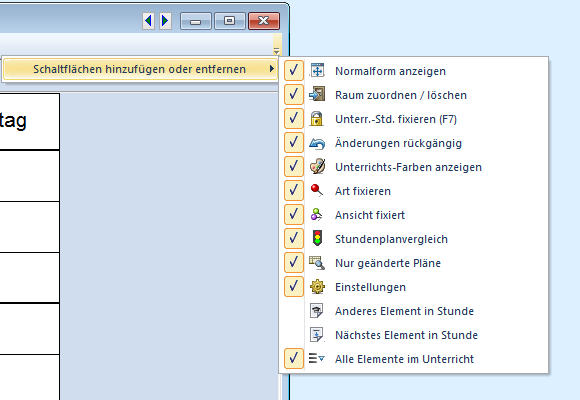
\includegraphics[width=.38\textwidth]{window-personalization}
	\vspace{-5pt}
	\caption{Fenster Personalisierung}
	\label{fig:window-personalization}
\end{wrapfigure}

Ab Untis 2015 sind die Symbolleisten der Fenster nicht mehr frei verschiebbar, dafür kann man sie ähnlich wie die Schnellzugriffs-Leiste, über der Pfeil nach unten an der rechten Seite der jeweilige Symbolleiste ein- oder ausblenden. Ein Klick auf den Pfeil öffnet ein Menü, dessen Länge von der Anzahl der nicht angezeigten Symbole abhängt. Wichtig ist hier der letzte Eintrag, \texttt{Schaltflächen hinzufügen oder entfernen}.\\
\\
Ein Klick auf den Eintrag, 'Schaltflächen hinzufügen oder entfernen' blendet ein weiteres Menü ein, mit welchem man die angezeigten Elemente nach Belieben anpassen kann. Zu berücksichtigen ist hierbei, dass die Elemente, die zur Auswahl stehen, vom jeweiligen Fenstertyp abhängig sind. Stammdaten-Fenstern stehen beispielsweise teilweise andere Bediensymbolen zur Verfügung, als Übersichtsplänen. Es ist sogar so, dass zwischen unterschiedlichen Fenstertypen unterschiedliche Funktionalität hinter den gleichen Symbolen steckt. Mehr Informationen dazu später in dieser und den ansichtsspezifischen Sektionen.\\
\\
Im ersten Teil des Abschnitts wird die überarbeitete Auswahlbox kurz erläutert. Danach werden die mit der Symbolleiste verbundenen Aktionen angesprochen, welche einfache Aktionen durchführen oder weitere Schnittstellen öffnen. Der Einfachheit halber wird die Symbolleiste 'Aktionen' benannt. Im dritten Teil werden Bedienfunktionen, welche erst mit der Eingabe und Anzeige von Daten einleuchten können, beschrieben, im Folgenden als Fenster-Aktionen benannt.

\subsection{Auswahl / Suche}

Die Auswahlbox in Untis Version 2015 wurde deutlich überarbeitet und bietet viele neue Verbesserungen. Die statische Auswahl wächst nun dynamisch in die Breite. Damit werden die, für gewöhnlich aussagekräftigeren, Langnamen immer angezeigt.\\

\begin{wrapfigure}{r}{.4\textwidth}
	\vspace{-13pt}
	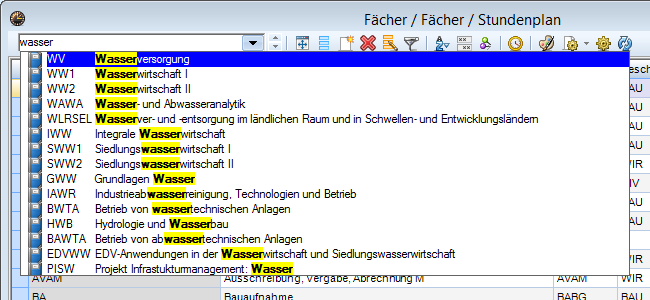
\includegraphics[width=.38\textwidth]{search-field}
	\vspace{-5pt}
	\caption{Suchen}
	\label{fig:search-field}
\end{wrapfigure}

\noindent
Die Auswahlbox als solche ist jedoch nebensächlich geworden, da beim Eintippen die kompletten Inhalte der Kurz- und Langnamen durchsucht werden. Bei der Eingabe eines einzelnen Zeichens grenzt Untis die Ergebnisse bereits ein und zeigt diese auch sofort in einer Drop-Down Liste an. Sprich, bei vielen Ressourcen ist es immer schneller, die Auswahlbox als Suchfeld zu verwenden. 

\subsection{Symbolleiste Aktionen}

Im Folgenden werden die typischen Symbole der Stammdaten-, Unterrichts- und Stundenplansansichten kurz erläutert. Für uns überflüssige Symbole werden nicht angesprochen.\\

\subsubsection{Alle Elemente im Unterricht}
{\small\textit{verfügbar in Einzelplan Ansichten\\}\par}

\begin{wrapfigure}{r}{.06\textwidth}
	\vspace{-50pt}
	
\includegraphics[width=.06\textwidth]{alle-elemente-im-unterricht-symbol}
	\vspace{-35pt}
\end{wrapfigure}

\noindent
Dieses Symbol erzeugt eine kleine Reiterleiste im oberen linken Eck eines Einzelplans. Falls man eine Unterrichtsstunde im Plan auswählt, werden Reiter erstellt und dieser Reiterleiste hinzugefügt. Man kann auf die Elemente dieser Leiste klicken um die Einzelpläne der verbundenen Ressourcen schnell anzuschauen. Standardmäßig eingeschaltet, lässt das Ausschalten einen Reiter verschwinden und, sollte man einen anderen Plan angeschaut haben, man bekommt den Ursprungsplan dargestellt.\\

\subsubsection{Änderungen Rückgängig}
{\small\textit{explizit verfügbar in allen Stundenplan-Ansichten\\}\par}

\begin{wrapfigure}{r}{.05\textwidth}
	\vspace{-50pt}
	
\includegraphics[width=.05\textwidth]{anderungen-ruckgangig-symbol}
	\vspace{-35pt}
\end{wrapfigure}

\noindent
Änderungen werden in Untis protokolliert und können rückgängig gemacht werden. Stundenpläne steht dieses Symbol in der Symbolleiste zur Verfügung. Ein Rückgängig-Befehl kann jedoch in jeder Ansicht verwendet werden. In den Ansichten, in welchen das Symbol nicht angezeigt wird, kann man auf die Tastenkombination STRG + Z zurückgreifen oder das Symbol in der Schnellzugriff Leiste betätigen.\\
\\
\textbf{Vorsicht}: \textit{Diese Funktion protokolliert im aktuellen Stand die zugewiesenen Räume in der Planung nicht mit! Manuell zugewiesene Räume gehen verloren!}\\

\subsubsection{Ansicht Fixiert}
{\small\textit{verfügbar in allen Fenster Ansichten\\}\par}

\begin{wrapfigure}{r}{.05\textwidth}
	\vspace{-50pt}
	
\includegraphics[width=.05\textwidth]{ansicht-fixiert-symbol}
	\vspace{-35pt}
\end{wrapfigure}

\noindent
Diese Aktion beeinflusst das Verhalten des Fensters in Abhängigkeit zu den ausgewählten Elementen anderer Fenster. Standardmäßig ist diese ausgestellt, sprich das Fenster wird von Benutzerinteraktion mit anderen Fenstern beeinflusst. Dies kann oft von Vorteil sein, z.B. wenn man Ressourcenpläne von unterschiedlichen Typen gleichzeitig untersucht. Sobald man die Pläne zweier Ressourcen des gleiche Ressourcentyps untersucht ist es ratsam einen dieser Pläne zu fixieren, da sich die ausgewählte Ressourcen sonst den Plänen anpassen..\\

\newpage

\subsubsection{Einstellungen}
{\small\textit{verfügbar in allen Fenster Ansichten\\}\par}

\begin{wrapfigure}{r}{.05\textwidth}
	\vspace{-50pt}
	
\includegraphics[width=.05\textwidth]{einstellungen-symbol}
	\vspace{-35pt}
\end{wrapfigure}

\noindent
Obwohl in allen Fenster-Ansichten verfügbar, verbirgt sich hinter dem Einstellungs-Symbol für jede Ansicht eine abweichende Funktionalität.\\
\\
Bei Stammdaten- und Unterricht-Ansichten sind die Einstellungen hauptsächlich auf die Auswahl der Schriftart, -größe und - stil begrenzt. Bei Unterrichts-Ansichten kann man zusätzlich entscheiden, ob die Summen-Zeile und geerbte Kennzeichen angezeigt werden sollen. Die Option ``nur eine Woche" scheint die Anzeige der Unterrichtstunden auf die Stunden, die in der erste Schulwoche stattfinden, einzugrenzen. Eine Möglichkeit weitere Wochen anzusehen, scheint nicht verfügbar zu sein. Diese Option sollte Ihrerseits nicht gesetzt werden.\\
\\
Bei Stundenplan-Ansichten öffnen sich weitere Einstellungen, welche später in Sektion !!!!!!! näher betrachtet werden.\\

\subsubsection{Elementart}
{\small\textit{verfügbar in Stundenplan-Ansichten\\}\par}

\noindent %this
Erlaubt einen direkt von einem Ressourcenart zu einem Anderen zu wechseln. Das Icon ist abhängig von der ausgewählte Ressourcentyp. Obwohl Studenten als Ressourcentyp zur Auswahl steht dieser scheint nicht implementiert zu sein, bitte nicht benutzen.

\subsubsection{Erweitertes Entkoppeln}
{\small\textit{verfügbar in Unterricht Ansichten\\}\par}

\begin{wrapfigure}{r}{.05\textwidth}
	\vspace{-50pt}
	
\includegraphics[width=.05\textwidth]{erweitertes-entkoppeln-symbol}
	\vspace{-35pt}
\end{wrapfigure}

\noindent
Dieses Symbol öffnet die Entkoppeln-Ansicht, zur Umgestaltung von ausgewählten Unterrichtskopplungszeilen zu eigenständigen Unterrichten. Mehr dazu in Sektion !!!!!!!.

\subsubsection{Farbe des Elements}
{\small\textit{verfügbar in Stammdaten- und Unterricht-Ansichten\\}\par}

\begin{wrapfigure}{r}{.05\textwidth}
	\vspace{-50pt}
	
\includegraphics[width=.05\textwidth]{farbe-des-elements-symbol}
	\vspace{-35pt}
\end{wrapfigure}

\noindent
Dieses Symbol öffnet die Farb-Ansicht. Hier kann man die Vorgrund- (Schrift) sowie Hintergrund-Farben von Elementen einstellen. Untis hat von Haus aus eine Palette mit 48 Farben und lässt bis zu 12 eigene Definitionen zu. Man kann die Farb-Einstellungen eines Elements einfach entfernen, in dem man ein Häkchen bei 'keine Farben' setzt. Sofern man die Ansicht noch nicht geschlossen hat, kann man die bisherigen Einstellungen durch das Entfernen des Häkchens wiederherstellen. Des Weiteren kann man Stammdaten-Elemente so einrichten, dass neu angelegte Elemente automatisch Farben zugewiesen bekommen.

\newpage

\subsubsection{Felder der Ansicht}
{\small\textit{verfügbar in Stammdaten- und Unterricht-Ansichten\\}\par}

\begin{wrapfigure}{r}{.05\textwidth}
	\vspace{-50pt}
	
\includegraphics[width=.05\textwidth]{felder-der-ansicht-symbol}
	\vspace{-35pt}
\end{wrapfigure}

\noindent
Untis verlangt von Haus aus nur das Nötigste an Informationen, um Daten anzulegen. Bei Stammdaten wird nur der \texttt{Name} (Kurzname) der Ressource und bei Unterrichten nur eine Anzahl der zu haltende Stunden benötigt. Jedoch hat jeder Ressourcentyp einen Standardsatz an Zusatzfeldern, welche standardmäßig eingeblendet sind. Diese sind für unsere Zwecke jedoch nicht ausreichend und ansatzweise auch nicht passend. 

\begin{wrapfigure}{r}{0.4\textwidth}
	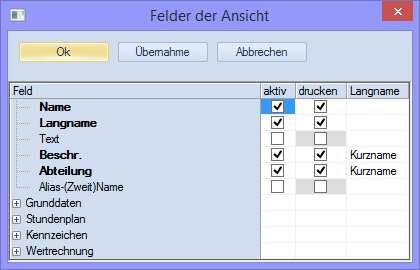
\includegraphics[width=.38\textwidth,right]{felder-der-ansicht}
	\vspace{-15pt}
	\caption{Felder der Ansicht}
	\label{fig:felder-der-ansicht}
	\vspace{10pt}
\end{wrapfigure}

\noindent
Damit wir möglichst aussagekräftige Daten haben im System, müssen die Felder erst angepasst werden. Diese werden über das Symbol, bzw. der Ansicht \texttt{Felder der Ansicht} eingeblendet. Hier kann man überflüssige Angaben, wie Hohlstunden, ausblendet und wichtige wie Schulübergreifender Name eingeblendet werden. Die spezifische Felder werden bei der jeweilige Ansicht näher erläutert.\\
\\
Sofern die Angabe eine weitere verwaltete Ressource ist, kann man auswählen wie die Angabe dieser Ressource erfolgen soll. Möglich sind der \texttt{Kurzname}, der \texttt{Langname} (bzw. \texttt{Nachname}) oder beide Namen mit einem Schrägstrich ``/" getrennt.\\

\subsubsection{Felder mit Inhalt}
{\small\textit{verfügbar in Stammdaten- und Unterricht-Ansichten\\}\par}

\begin{wrapfigure}{r}{.05\textwidth}
	\vspace{-50pt}
	
\includegraphics[width=.05\textwidth]{felder-mit-inhalt-symbol}
	\vspace{-35pt}
\end{wrapfigure}

\noindent
Felder mit Inhalt blendet \textbf{alle} mit einem Wert belegten Felder ein. Dies kann hilfreich sein, um sich daran zu erinnern welche Felder mit Werten zu belegen sind. Es kann auch ein etwas tieferes Verständnis der Abläufe in Untis verschaffen, da neben den vom Benutzer eingegebenen Werte auch die dynamisch vom Programm berechneten werte angezeigt werden.\\

\subsubsection{Fenster Aktualisieren}
{\small\textit{verfügbar in Stammdaten- und Unterricht-Ansichten\\}\par}

\begin{wrapfigure}{r}{.05\textwidth}
	\vspace{-50pt}
	
\includegraphics[width=.05\textwidth]{felder-mit-inhalt-symbol}
	\vspace{-35pt}
\end{wrapfigure}

\noindent
Dieses Symbol aktualisiert das Fenster. Untis sucht nach lokalen und externen Änderungen und pflegt gefundene Datensätze sortiert ein.\\

\newpage

\subsubsection{Klassenzeitraster}
{\small\textit{verfügbar in Gruppen-Stammdaten Ansichten\\}\par}

\begin{wrapfigure}{r}{.05\textwidth}
	\vspace{-50pt}
	
\includegraphics[width=.05\textwidth]{klassenzeitraster-symbol}
	\vspace{-35pt}
\end{wrapfigure}

\noindent
Hier wird ein Fenster geöffnet, in dem man den Tagesablauf einer Gruppe anhand der assoziierten Raster für die automatische/optimierte Planung festlegen kann. Da dieses nicht vollständig implementiert zu sein scheint, sollten Sie es nicht benutzen.\\

\subsubsection{Koppeln}
{\small\textit{verfügbar in Unterricht Ansichten\\}\par}

\begin{wrapfigure}{r}{.05\textwidth}
	\vspace{-50pt}
	
\includegraphics[width=.05\textwidth]{koppeln-symbol}
	\vspace{-35pt}
\end{wrapfigure}

\noindent
Dieser Symbol öffnet eine Ansicht, in welcher mehrere getrennte Unterrichte zu einem Unterricht mit mehreren Kopplungszeilen zusammenfügt werden kann. Nähere Informationen dazu in Sektion !!!!!!!.\\

\subsubsection{Lehrer-Vorschlag}
{\small\textit{verfügbar in Unterricht Ansichten\\}\par}

\begin{wrapfigure}{r}{.06\textwidth}
	\vspace{-50pt}
	
\includegraphics[width=.06\textwidth]{lehrer-vorschlag-symbol}
	\vspace{-35pt}
\end{wrapfigure}

\noindent
Der Lehrer-Vorschlag bietet Ihnen ein kleines Menü, in welchem die Möglichkeiten der Lehrer-Vorschlags-Ansicht (das Leeren des Dozent-Feldes, Verwendung des Vorjahres-Lehrer) aufgelistet sind.\\
\\
Die Lehrer-Vorschlag-Ansicht listet alle Dozenten anhand ihrer von Untis eingetragenen/kalkulierten Ist, Soll und Ist-Soll Werte auf. Diese kann von nutzen sein wenn man nach einem Dozenten mit freien Kapazitäten sucht. Standardmäßig werden die Dozenten nach ihren noch zu führenden Stunden aufgelistet, jedoch können diese Angaben nach allen Spalten sortiert werden.\\
\\
Die Option Vorjahres-Lehrer bezieht sich auf Klassen-Lehrer wie man sie von der Grundschule oder dem Gymnasium kennt und ist für unsere Zwecke nicht zu gebrauchen.\\

\subsubsection{Löschen}
{\small\textit{verfügbar in Stammdaten- und Unterricht-Ansichten\\}\par}

\begin{wrapfigure}{r}{.05\textwidth}
	\vspace{-50pt}
	
\includegraphics[width=.05\textwidth]{loschen-symbol}
	\vspace{-35pt}
\end{wrapfigure}

\noindent %this
Entfernt alle markierte Einträge von der aktuelle Periode. Die Einträge können weiterhin in andere Perioden bestehen.

\newpage

\subsubsection{Normalform Anzeigen}
{\small\textit{verfügbar in allen Fenster Ansichten\\}\par}

\begin{wrapfigure}{r}{.05\textwidth}
	\vspace{-50pt}
	
\includegraphics[width=.05\textwidth]{normal-form-anzeigen-symbol}
	\vspace{-35pt}
\end{wrapfigure}

\noindent
Die Schaltfläche Normalform Anzeigen bewirkt, dass die Breite des Fensters sich der Höhe und Breite der angezeigten Zeilen und Spalten anpasst. Bei eine geringen Anzahl an Einträgen wird die Höhe des Fensters ggf. schrumpfen. Wohingegen bei vielen Zeilen jedoch die komplette Höhe der Arbeitsfläche eingenommen werden könnte.\\
\\
Zusätzlich führt das Klicken auf dieses Symbol bei manchen Ansichten eine Art Zurücksetzen durch. Bei Gruppenstundenplänen zum Beispiel wird man zurück zum Gruppenplan vom letzten angeklickten Unterricht geführt. Dies kann eine ganz andere Gruppe sein als jene, mit der man angefangen hat.\\

\subsubsection{Nur geänderte Pläne}
{\small\textit{verfügbar in Stundenplan-Ansichten\\}\par}

\begin{wrapfigure}{r}{.05\textwidth}
	\vspace{-50pt}
	
\includegraphics[width=.05\textwidth]{nur-geanderte-plane-symbol}
	\vspace{-35pt}
\end{wrapfigure}

\noindent %this paragraph
Diese Funktion soll der Vergleich zwischen zweier Pläne auf das Geänderte einschränken. Da der Vergleich-Funktion nicht funktioniert könnte ich das nicht ausprobieren.

\subsubsection{Raum Zuordnen / Löschen}
\label{subsubsec:raum-zuordnen-loschen}
{\small\textit{verfügbar in Unterricht Ansichten\\}\par}

\begin{wrapfigure}{r}{.05\textwidth}
	\vspace{-50pt}
	
\includegraphics[width=.05\textwidth]{raum-zuordnen-loschen-symbol}
	\vspace{-35pt}
\end{wrapfigure}

\noindent
Dieses Symbol, oder der entsprechende Unterrichtsstunden-Kontextmenüeintrag, öffnet die Ansicht \texttt{Raum zuordnen / löschen} für die im Stundenplan selektierte Stunde. Hier kann man alle Räume einer Periode, mit ausgewählten Informationen wie \texttt{Besetzt} (ob der Raum schon in der Stunde verplant ist), \texttt{Kapazität} (Anzahl der Sitzplätze), ob ein Raum als \texttt{Ausweichraum} für den gewünschten Raum eingetragen ist, sowie die Raumgruppenzugehörigkeit, sehen.\\

\begin{wrapfigure}{r}{0.3\textwidth}
	\vspace{-14pt}
	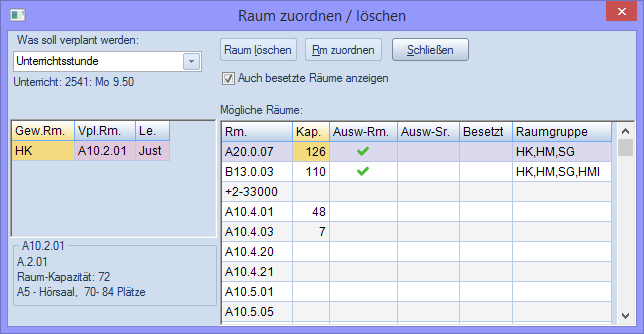
\includegraphics[width=.29\textwidth,right]{raum-zuordnen-loschen}
	\vspace{-15pt}
	\caption{Raum zuordnen / löschen}
	\label{fig:raum-zuordnen-loschen}
\end{wrapfigure}

\noindent %here until the end of the subsubsection
Man kann Raume zuordnen, indem man einen Raum selektiert und den Knopf \texttt{Rm zuordnen} drückt, oder  zwei mal auf den gewünschten Raum klickt. Man kann auf ähnlicher Weise die Zuordnung löschen in dem man \texttt{Raum löschen} drückt oder zwei mal auf den nicht erwünschten Raum klickt.\\
\\
Besetzte Räume werden mit einem Häkchen dargestellt in der entsprechende Spalte. Als dieser Ansicht geöffnet wird werden solche Räume entweder unten an der Liste der Räume angehängt oder gar ausgeblendet. Falls zweites eintreffen sollte muss man ein Häkchen bei \texttt{Auch besetzte Räume Anzeigen} um diese einzublenden. Auch wenn Räume besetzt sind kann man dennoch Unterrichtsstunden zugewiesen werden wie oben beschrieben. Diese Zuordnung bringt eine weitere Warnungs- /Bestätigunsansicht hoch \texttt{Raum nicht frei}.\\

\begin{wrapfigure}{r}{0.3\textwidth}
	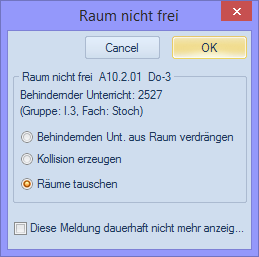
\includegraphics[width=.29\textwidth,right]{raum-nicht-frei}
	\vspace{-15pt}
	\caption{Raum nicht frei}
	\label{fig:raum-nicht-frei}
	\vspace{10pt}
\end{wrapfigure}

\noindent
\texttt{Raum nicht frei} gibt eine kurze Auflistung der Unterrichte die durch diese Raumbelegung betroffen wären sowie drei Optionen wie dieser Konflikt gelöst werden könnte: \texttt{Behinderten Unt. aus Raum verdrängen} (andere Unterrichte verlieren ihre Raumzuordnung), \texttt{Kollision erzeugen} (alle Unterrichte behalten ihre Zuordnung und der neue kommt dazu) und \texttt{Räume tauschen} (andere Unterrichte bekommen die vorherige des aktuellen Unterrichts). Alle drei haben ihre situationsbedingte Einsatz, normalerweise ist \texttt{Kollsion erzeugen} ein sichere Wahl vorausgesetzt man geht bewusst mit der Erzeugung von Kollisionen um. Unten gibt es eine weitere Einstellungsmöglichkeit, \texttt{Diese Meldung dauerhaft nicht mehr anzeig...}, das setzten dieses Häkchen bewirkt, dass der \texttt{Raum nicht frei} Ansicht nicht mehr zum Vorschein kommt. Bisher habe ich keine Möglichkeit gefunden diese wieder anzeigen zu lassen. \textbf{Bitte setze nicht das Häkchen.}

\subsubsection{Schuljahreskalendar}
{\small\textit{verfügbar in Stammdaten (ausser Fächer) und Unterricht Ansichten\\}\par}

\begin{wrapfigure}{r}{.05\textwidth}
	\vspace{-50pt}
	
\includegraphics[width=.05\textwidth]{schuljahreskalendar-symbol}
	\vspace{-35pt}
\end{wrapfigure}

\noindent
Bei Stammdaten öffnet dieses Symbol die Absenzen-Ansicht, in welcher man die nicht verfügbaren Tage einer Ressource eintragen kann. Leider scheint diese Funktion nicht vollständig implementiert zu sein und ist an mehreren Stellen fehlerhaft, weshalb sie nicht benutzt werden sollte.\\
\\
Bei Unterrichten wird tatsächlich der Schuljahreskalender geöffnet. Hier wird der Ablauf des Unterrichts, abhängig vom Unterrichtsgruppe (Von- und Bis- Datum), angezeigt. Der Verlauf lässt sich jedoch nicht von dieser Ansicht beeinflussen.\\

\subsubsection{Seitenlayout}
{\small\textit{verfügbar in Stammdaten- und Unterricht-Ansichten\\}\par}

\begin{wrapfigure}{r}{.06\textwidth}
	\vspace{-50pt}
	
\includegraphics[width=.06\textwidth]{seitenlayout-symbol}
	\vspace{-35pt}
\end{wrapfigure}

\noindent
Ein Klick auf dieses Symbol öffnet ein kleines Menü mit dem Punkten Seitenansicht und Seitenlayout. Seitenansicht beschreibt die druckbare Ausgabe der in dem Fenster erhaltenen Informationen, wohingegen Seitenlayout dessen Gestaltungseinstellungen beinhaltet. Mehr Informationen dazu finden Sie in Sektion !!!!!!.

\subsubsection{Sortieren (automatische)}
{\small\textit{verfügbar in Stammdaten- und Unterricht-Ansichten\\}\par}

\begin{wrapfigure}{r}{.05\textwidth}
	\vspace{-50pt}
	
\includegraphics[width=.05\textwidth]{sortieren-symbol}
	\vspace{-35pt}
\end{wrapfigure}

\noindent
Das Sortieren-Symbol öffnet eine weitere Ansicht, welche das automatische Sortieren ermöglicht. Hier können mehrere Spalten ausgewählt werden, welche als Sortier-Kriterien dienen können. Außerdem kann die Sortierrichtung der Kriterien bestimmt werden.\\

\begin{wrapfigure}{r}{0.3\textwidth}
	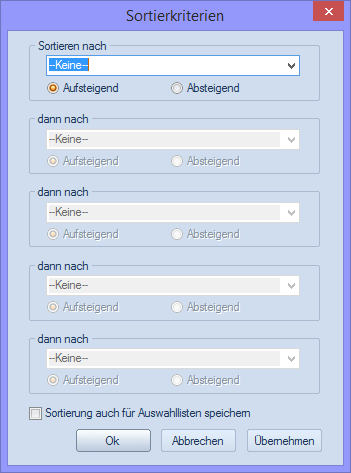
\includegraphics[width=.29\textwidth,right]{sortierkriterien}
	\vspace{-15pt}
	\caption{Sortierkriterien}
	\label{fig:sortierkriterien}
\end{wrapfigure}

\noindent
Das eingestellte Sortierverhalten kann mit \texttt{Ok} oder \texttt{Übernahme} bestätigt werden. Obwohl das Verhalten \textit{permanent} gespeichert wird, kann es nach dem Schließen des Fensters nicht nochmal eingesehen werden. Sollte die Sortierkriterien-Ansicht nach dem Schließen neu aufgerufen werden, werden keine der bereits gespeicherten Einstellungen angezeigt und, sollte man sie nicht neu einstellen, gehen sie nach dem Schließen der Ansicht immer verloren.\\
\\
Für Ansichten, die mit Stammdaten assoziiert sind, kann man unten in der Ansicht ein Häkchen setzen, welches bewirkt, dass die gespeicherte Sortierung auch für Auswahlboxen für den Ressourcentyp eingehalten wird. Jedoch egal in welchem Zustand sich das Sortieren befindet, müssen neue Elemente manuell-automatisch eingerichtet werden. Sprich die Sortierung muss neu mit Häkchen eingestellt werden, damit die gewünschte Sortierung neue Elemente in den Auswahlboxen berücksichtigt.\\

\subsubsection{Stundenplanvergleich}
{\small\textit{verfügbar in Stundenplan-Ansichten\\}\par}

\begin{wrapfigure}{r}{.05\textwidth}
	\vspace{-50pt}
	
\includegraphics[width=.05\textwidth]{stundenplan-vergleich-symbol}
	\vspace{-35pt}
\end{wrapfigure}

\noindent
Dieser Symbol soll es ermöglichen zwei Stundenpläne zu vergleichen. Laut dem Tooltip soll Untis deswegen ein zweites mal gestartet werden. Diese Funktion hat bei jedem klick verursacht, dass das Programm sich aufgehalten hat. Bitte nicht verwenden.\\

\subsubsection{Unterrichtsstunde Fixieren}
{\small\textit{verfügbar in Stundenplan-Ansichten\\}\par}

\begin{wrapfigure}{r}{.05\textwidth}
	\vspace{-50pt}
	
\includegraphics[width=.05\textwidth]{unterrichtsstunde-fixieren-symbol}
	\vspace{-35pt}
\end{wrapfigure}

\noindent
Sollte man die automatische/optimierte Planung verwenden, verhindert das Betätigen dieses Symbols, dass der geplante Unterricht von diesen Planungsvorgängen geändert wird.\\

\subsubsection{Unterrichtsvergleich}
{\small\textit{verfügbar in Unterricht Ansichten\\}\par}

\begin{wrapfigure}{r}{.05\textwidth}
	\vspace{-50pt}
	
\includegraphics[width=.05\textwidth]{unterrichtsvergleich-symbol}
	\vspace{-35pt}
\end{wrapfigure}

\noindent
Durch dieses Symbol lassen sich Unterrichte mit der selben ID unterschiedlicher Perioden vergleichen. Einmal angeklickt, öffnet sich eine Ansicht, in welcher man die Periode, sowie die Darstellung der Ergebnisse auswählen kann. Da wir mit viel Fluktuation in der Zahl der Studenten, angebotenen Fächer, Studentengruppen und eingesetzten Dozierenden umgehen müssen, bringt uns diese Funktion nicht viel.\\

\subsubsection{Zeitwünsche}
{\small\textit{verfügbar in Stammdaten- und Unterricht-Ansichten\\}\par}

\begin{wrapfigure}{r}{.05\textwidth}
	\vspace{-50pt}
	
\includegraphics[width=.05\textwidth]{zeitwunsche-symbol}
	\vspace{-35pt}
\end{wrapfigure}

\noindent
Zeitwünsche öffnet ein weiteres Fenster, in welchem man Präferenzen zu den Zeiten, in denen Stammdaten zur Verfügung stehen oder Unterrichte gehalten werden sollen, angeben kann. Diese Präferenzen sind abgebildet auf numerische Werte zwischen -3 und +3 mit einem großen 'X' anstelle der 0 Im Wesentlichen dienen diese Angaben der automatischen/optimierten Stundenplanerstellung. Doch die Angabe -3 hat einen besonderen Stellenwert, da er als absolute Sperre gilt. Einst belegt mit diesem Wert, wird Untis, sobald man manuell versucht einen Unterricht zu einer gesperrten Zeit zu planen, einen Fehler melden.\\
\\

\begin{wrapfigure}{r}{0.3\textwidth}
	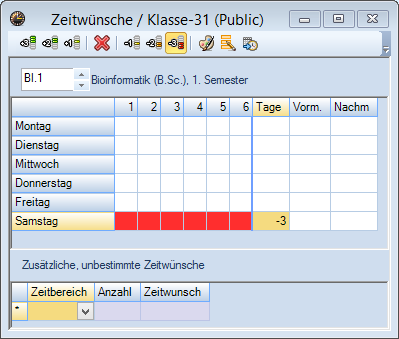
\includegraphics[width=.29\textwidth,right]{zeitwunsche-gruppen}
	\vspace{-15pt}
	\caption{Zeitwünsche Gruppen}
	\label{fig:zeitwunsche-gruppen}
\end{wrapfigure}

\noindent
Die Zeitwünsche-Ansichten haben ein paar wesentliche Binnendifferenzen in Abhängigkeit zur aufrufenden Ansicht, ggf. dessen Ressourcentyp und der Verwendung der sogenannten Multi-Zeitraster. In \figref{fig:zeitwunsche-gruppen} sehen wir die Zeitwünsche- Ansicht für die Ressource Gruppen. Im Hauptteil des Fensters steht mittig das Zeitraster des Elements. Hier kann man die Werte blockweise Eintragen, in denen Unterrichte für diese Ressource stattfinden, bzw. nicht-stattfinden sollen. Bei Gruppen- und Dozenten-Zeitwünschen hat man Zugriff auf erweiterte Hilfsmittel zu Setzen von Werten für ganze Zeitbereiche (Ganztags, Vormittags oder Nachmittags). Räume- und Fächer-Zeitwünsche haben kein solches Hilfsmittel.\\
\\
Da Gruppen immer an ein festes Zeitraster gebunden sind, wird dieses immer in der entsprechenden Zeitwünsche-Ansicht angezeigt. Bei Dozenten, Räumen und Fächern hingegen kann kein eindeutiges Zeitraster angegeben werden. Sollten mehrere Raster vorliegen, sehen ihre Zeitwünsche komplizierter aus, wie in \figref{fig:zeitwunsche-multiraster} veranschaulicht. Hier muss man entsprechende Zeitbereiche mit dem jeweiligen Wert belegen. Die aktuelle Position des Cursors (in Minuten) wird in der ersten Reihe/Spalte angezeigt.

\begin{figure}[h]
	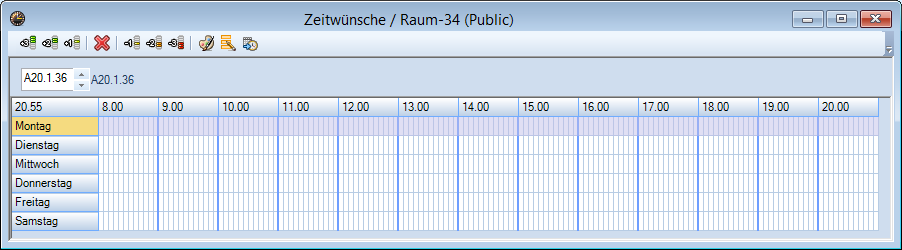
\includegraphics[width=1\textwidth]{zeitwunsche-multiraster}
	\vspace{-15pt}
	\caption{Zeitwünsche Multi-Zeitraster}
	\label{fig:zeitwunsche-multiraster}
\end{figure}

\begin{wrapfigure}{r}{0.3\textwidth}
	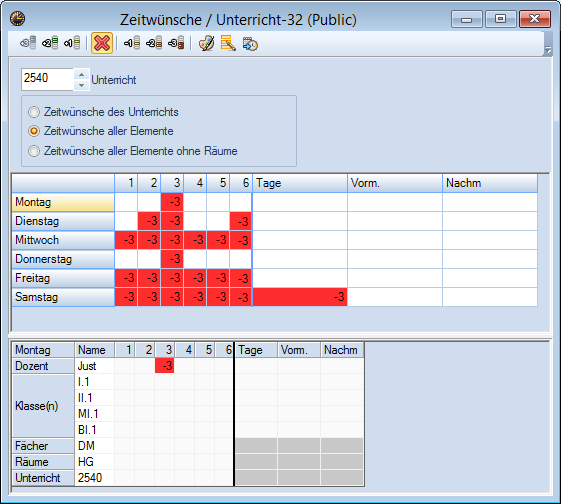
\includegraphics[width=.29\textwidth,right]{zeitwunsche-unterricht}
	\vspace{-15pt}
	\caption{Zeitwünsche Unterrichte}
	\label{fig:zeitwunsche-unterricht}
\end{wrapfigure}

\noindent
Unterrichte sind über die zugewiesenen Klassen auch an ein festes Raster gebunden und wie Gruppen und Dozenten kann man auch ganze Zeitbereiche mit einem Wert belegen. Man hat hier die Wahl zwischen drei verschiedenen Darstellungsmöglichkeiten: Unterricht, alle Elemente und alle Elemente ohne Räume. Bei allen drei Möglichkeiten werden automatisch die Zeitwunsch-Werte der assoziierten Ressourcen tageweise unten dargestellt. In \figref{fig:zeitwunsche-unterricht} z.B. sieht man in der Liste der Ressourcen unten eine Sperre bei Frau Just Montags im 3. Block. Bei \texttt{alle Elemente} und \texttt{alle Elemente ohne Räume} werden die Zeitwünsche der assoziierten Ressourcen direkt als die des Unterrichts angezeigt. 

\subsection{Fenster-Aktionen}

\subsubsection{Filter}%everything from here on
{\small\textit{verfügbar in Stammdaten- und Unterricht-Ansichten\\}\par}

\begin{wrapfigure}{r}{.05\textwidth}
	\vspace{-50pt}
	
\includegraphics[width=.05\textwidth]{filter-symbol}
	\vspace{-35pt}
\end{wrapfigure}

\noindent
Filtern ermöglicht das Einschränken der angezeigten Einträge nach der eingetragenen Werte einer Spalte. Man klickt auf das Filter-Symbol um das Filtern zu aktivieren. Danach erscheint ein neue Zeile als erster Eintrag in der Tabelle. Hier trägt man in der Spalte nach dem gesucht wird einen Wert ein. Prinzipiell gilt der ganze Wert, es kann aber nach der Anfang des Werts gesucht werden. Zum Beispiel, sollte man im Langname-Spalte der Filterzeile von Raumstammdaten 'A20.*' wäre die Liste auf alle Räume in Gebäude A20.

\subsubsection{Neu}
{\small\textit{verfügbar in Stammdaten- und Unterricht-Ansichten\\}\par}

\begin{wrapfigure}{r}{.05\textwidth}
	\vspace{-50pt}
	
\includegraphics[width=.05\textwidth]{neu-symbol}
	\vspace{-35pt}
\end{wrapfigure}

\noindent
Das Klicken des Neu-Symbols bringt der Fokus zum ersten Spalte der letzten Zeile des Fensters. Man kann auch selber dahin scrollen. Welche Daten einzupflegen sind wird in die \chapref{chap:data}, und \chapref{chap:lessons}, näher erläutert.\\

\subsubsection{Serien-Änderung} 
{\small\textit{verfügbar in Stammdaten- und Unterricht-Ansichten\\}\par}

\begin{wrapfigure}{r}{.05\textwidth}
	\vspace{-50pt}
	
\includegraphics[width=.05\textwidth]{serien-anderung-symbol}
	\vspace{-35pt}
\end{wrapfigure}

\noindent
Serienänderungen sind Änderungen die auf einem bestimmten Bereich oder Einzeleinträge einer Spalte ausgeführt werden. Diese Funktionalität kann sehr behilflich sein bei der Pflege von neuen Informationen, oder das löschen von nicht verwendete/gewollte Attribute. Man kann diese Funktionalität mit oder ohne die vorgesehene Schnittstelle ausführen. Beide Möglichkeiten haben ihre stärken und setzen Interaktion mit dem Listenbereich des Fensters voraus, denn die zu ändernde Einträge müssen erst ausgewählt werden.\\
\\
Einzeleinträge werden durch mehrfaches STRG + Klick ausgewählt. Bereiche können mit dem Streichen der Maus oder in dem man einen Eintrag auswählt und UMSCHALT + Klick auf den letzten im gewünschten Bereich macht. Die Methode um einen Bereich zu markieren ist auch nachher mit der Methode um Einzeleinträge kombinierbar, aber nicht anders herum.\\

\begin{figure}[h]
	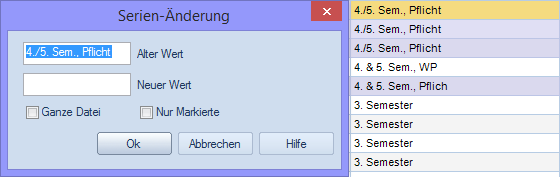
\includegraphics[width=1\textwidth]{serien-anderung}
	\vspace{-15pt}
	\caption{Serien Änderung}
	\label{fig:serien-anderung}
\end{figure}

\noindent
Im \figref{fig:serien-anderung} habe ich vier Felder markiert. Ich kann nach dieser Markierung direkt einen neuen Wert eintragen die in allen markierten Felder übernommen wird. Darüber hinaus bietet mir die \texttt{Serien-Änderung} Schnittstelle viele weiter Möglichkeiten. In der Ansicht reicht es vollkommen aus nur einen Feld auszuwählen, denn standardmäßig werden alle angezeigte Werte der Spalte miteinbezogen. Man kann diese ausdehnen in dem man ein Häkchen bei \texttt{Ganze Datei} setzt, diese beeinflusst auch die, durch Filteriren, ausgeblendete Werte. Der Einflussbereich kann man auch durch Markieren und den Auswahl von \texttt{Nur Markierte} ebenso gut einschränken. Sofern ein Wert in \texttt{Alter Wert} eingetragen ist werden nur die Einträge, in den dieser Wert vorkommt, durch den neuen Wert geändert. 

\subsubsection{Sortieren (manuell)}
{\small\textit{implizti verfügbar in Stammdaten- und Unterricht-Ansichten\\}\par}

\noindent
Zusätzlich zum Automatischen sortieren gibt es zwei arten von manuelle Sortierung. Erstens kann man einzelne Zeilen per Drag \& Drop in der gewünschte Reihenfolge anbringen. Die hierdurch erzeugte Sortierung wird nachhaltig gespeichert. Man kann auch die Spaltennamen anklicken, diese sortiert die Einträge klein nach groß nach der Werte die in dieser Spalte eingetragen sind. Weitere Klicks ändern die Sortierrichtung. Diese Methode sortiert die vorhandene Einträge nur vorübergehend.

\chapter{Stammdatenpflege}
\label{chap:data}

\section{Stammdatenpflege}

\subsection{Planungsabschnitte (Perioden)}

Planungsabschnitte werden mit der Ressource \texttt{Perioden} in Untis modelliert. Diese Ressourcen sind bereits eingepflegt. Man kann zwischen den jeweiligen Perioden mittels eine Auswahlbox in der obere Menüleiste zwischen den jeweiligen Perioden wechseln. Die Semester sind in der Regel der Hauptplanungsabschnitt an der THM, das Schuljahr hingegen ist für die Pflege von Stammdaten gedacht.\\

\begin{wrapfigure}{r}{0.25\textwidth}
	\vspace{-14pt}
	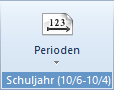
\includegraphics[width=.24\textwidth,right]{perioden}
	\vspace{-15pt}
	\caption{Perioden}
	\label{fig:mf-sg}
\end{wrapfigure}

\noindent
\textbf{Die Pflege der Stammdaten von Gruppen, Räume und Dozenten muss in der Periode ``Schuljahr" gemacht werden.} Wenn Daten in der Schuljahr-Periode eingepflegt sind, werden die neuen Daten, bzw. Änderungen, automatisch im Winter- und Sommersemester Perioden ersichtlich. Sollten neue Stammdaten oder Änderungen an bestehenden in die Winter- oder Sommersemester Perioden eingepflegt werden, sind diese Daten nur in diese eine Periode ersichtlich. Das führt zwangsläufig zu Dateninkonsistenzen.

\subsection{Name und Langname}

Bei einzelne Datensätze ist \texttt{Name} ein eindeutiger Schlüsselwert, der z.B. das schnelle eintippen dieser Ressource in Untis ermöglicht. Er soll dementsprechend so kurz und aussagekräftig wie möglich, gehalten werden. Der \texttt{Langname}, bzw. \texttt{Nachname}, hingegen enthält den tatsächlichen Namen der jeweilige Ressource. \textbf{Bei einzelne Datensätze sind Name und Langname immer Pflicht}.

\newpage

\subsection{Externer Name}
\label{sec:ext-name}

\texttt{Ext. Name} ist ein fachbereichsübergreifender Schlüsselwert. Er ermöglicht die Sicht auf die Planung der Ressource außerhalb des eigenen Fachbereiches. Für Räume ist diese Angabe Pflicht. Gruppen und Dozenten, die für fachbereichsübergreifende Planungen eingesetzt werden (wie z.B. im Studiengang Bioinformatik, SuK Veranstaltungen bei ME, oder Dozenten aus den Dienstleistungsfachbereichen) sollten ebenfalls einen solchen externer Name haben. Sollte eine benötigte Ressource noch nicht in den Stammdaten eines Fachbereiches eingetragen sein, so schicken Sie mir bitte ein Email - ich werde die diese Ressource dann zentral einpflegen und freigeben.

\section{Spezielle Ressourcen}

Spezielle Ressourcen sind solche, die nur als Attribute für andere Ressourcen verwendet werden: Studiengänge und Beschreibungen. Die Stammdatenpflege dieser Ressourcen erreicht man am leichtesten, indem man \texttt{Dateneingabe} in der Reiterleiste auswählt, \texttt{Sonstige Daten} aufklappt und \texttt{Studiengänge} oder \texttt{Beschreibungen} auswählt.\\

\begin{figure}[h]
	\centering
	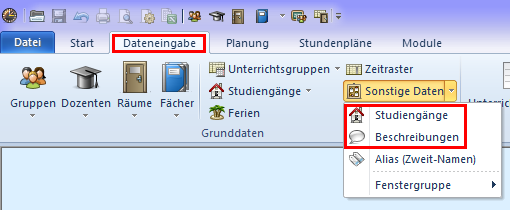
\includegraphics[width=.8\textwidth]{spezielle-daten-menu}
	\vspace{-5pt}
	\caption{Menüführung: spezielle Daten}
	\label{fig:spezielle-daten-menu}
\end{figure}

\subsection{Studiengänge (Abteilungen)}

Studiengänge werden an der THM Gruppen zugeordnet. Die damit implizierte Aussage ist: Gruppen gehören Studiengänge. Man könnte auch Dozenten, Räume und Fächer Studiengänge zuordnen. Dies würde wegen unserer weiteren Modellierung keine weitere Auswirkung haben und ist daher nicht nötig.\\
\\
THM Organizer verwendet Studiengänge um die Navigation für Gruppenpläne zu gestalten.\\

\newpage

\begin{wrapfigure}{r}{0.4\textwidth}
	\centering
	\vspace{-4pt}
	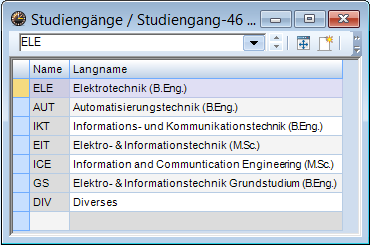
\includegraphics[width=.38\textwidth]{studiengange}
	\vspace{-5pt}
	\caption{Studiengänge}
	\label{fig:studiengange}
\end{wrapfigure}

\noindent
\texttt{Name}: Der Name besteht aus wenigen aber aussagekräftigen Buchstaben. Existiert der Studiengang als Bachelor und Master-Studiengang, so werden diese, getrennt durch einen Punkt, mit ``B" \hspace{1pt} bzw. ``M" \hspace{1pt} erweitert (Bsp.: Informatik Bachelor bzw. Master:  I.B bzw. I.M).\\

\noindent
\texttt{Langname}: Der Name des Studiengangs mit offizieller Abkürzung des Abschlusses in runden Klammern dahinter. Dieser Wert wird öffentlich verwendet in die Darstellungen von Untis und THM Organizer.

\subsection{Beschreibungen}

An der THM wird diese Ressource verwendet, um Fachkompetenzen, Raumkategorien und Unterrichtsmethoden zu modellieren. In Untis gibt es teilweise ähnliche Angaben, sie lassen sich aber nicht einstellen und sind deshalb für unsere Zwecke nicht verwendbar.\\
\\
Sollte diese Angabe bei der Dozent, Raum oder Fach fehlen wird der Plan nicht in der Navigation in Organizer erscheinen.\\

\noindent
{\large Attribute\par}
\vspace{8pt}

\begin{wrapfigure}{r}{0.4\textwidth}
	\centering
	\vspace{-14pt}
	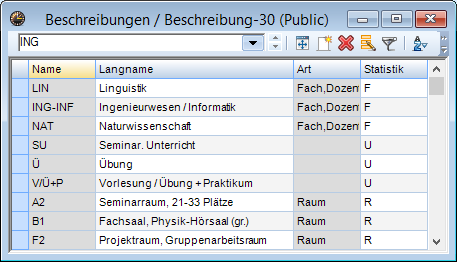
\includegraphics[width=.38\textwidth,right]{beschreibungen}
	\vspace{-15pt}
	\caption{Beschreibungen}
	\label{fig:beschreibungen}
	\vspace{-35pt}
\end{wrapfigure}

\noindent
\texttt{Art}: Diese Angabe ist für uns unbrauchbar und lässt sich leider nicht ausblenden. Daher bitte ignorieren.\\

\noindent
\texttt{Statistik}: Diese Angabe ist Pflicht und wird verwendet, um die Verwendung der Ressource festzulegen.\\

\vspace{9pt}

\subsubsection{Fachkompetenzen}
\label{subsec:fachkompetenzen}

Die Angabe zu den Fachkompetenzen gibt eine grobe Zuordnung der Ressourcen zu bestimmten fachlichen Bereichen vor.\\
\\
Derzeit sind die Namen und Langnamen nach einem von Herr Kneisel entworfenes System aufgebaut. Demnach besteht ein Fachkompetenz aus Basis-Kompetenzen, die jeweils durch drei Buchstaben gekennzeichnet sind. Diese entsprechen einem recht groben Themengebiet wie Naturwissenschaft oder Bauingenieurwesen. Zusätzlich gibt es die Möglichkeit, kombinierte Kompetenzen zu verwenden. Deren Namen setzen sich aus den Bezeichnern von zwei Basis-Kompetenzen, verbunden durch einen Bindestrich zusammen. Ihr Langname ergibt sich durch die Langnamen der Basis-Komponenten, getrennt durch einen Schrägstrich ``/". Fachkompetenzen sind in der Spalte \texttt{Statistik} durch den Buchstaben ``F" \hspace{1pt} gekennzeichnet.\\

\begin{quote}
	\textit{Hier wäre eine Überarbeitung des Systems grundsätzlich wünschenswert. Beispielsweise hat Fachbereich Wirtschaft, zusätzlich zu den Einträgen vom Kneisel'sche System, neun Schwerpunkte, wie Mittelstand oder Marketing. Diese sind um einiges aussagekräftiger und relevanter sowohl für Studenten als auch für Dozenten.}
\end{quote}

\noindent
THM Organizer verwendet diese Angaben für die Stundenplan-Navigation für Dozenten und Fächer, sowie die für die Gruppierung von Fächer im Modulhandbuch.

\subsubsection{Raumkategorien}
\label{subsec:room-category}

Der Name und der Langname beziehen sich auf einem System, entwickelt von Herr Deniffel für die THM, wonach die Namen den Raumtyp und Aussagen über dessen Kapazität oder Ausstattung kodieren.\\
\\
Der Name besteht meist aus einer Buchstabe und einer Zahl. ``A" steht beispielsweise für einen  Seminarraum oder Hörsaal, wohingegen ``D" ein Rechnerraum kennzeichnet. Die Zahlen beziehen sich auf Raumeigenschaften wie Größe oder Ausstattung. Bei A2 heißt das ``2" 21 bis 33 Sitzplätze, bei D2 hingegen heißt die ``2", dass sich in dem Raum eine fachspezifische Ausstattung befindet. Der Langname ist eine von Kommata getrennte Auflösung dieser zwei Teile. Bei Raumkategorien wird ein ``R" in der Statistik Spalte eingetragen.\\
\\
Eine vollständige Liste der Raumkategorien befindet sich im \secref{sec:dennifel}.\\
\\
THM Organizer verwendet diese Angaben für die Stundenplan-Navigation für Räume.\\

\subsubsection{Unterrichtsmethoden}

Unterrichtsmethoden beschreiben die Lehrform eines Unterrichts.\\

\begin{wrapfigure}{r}{0.35\textwidth}
	\vspace{-14pt}
	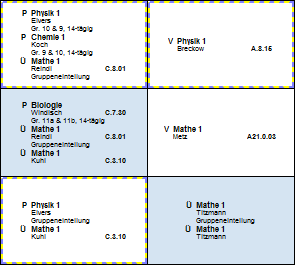
\includegraphics[width=.34\textwidth]{MethodsUntis}
	\vspace{-5pt}
	\caption{Mögliche Darstellung von Unterrichtsmethoden in Untis}
	\label{fig:methoden-untis}
	\vspace{-5pt}
\end{wrapfigure}

\noindent
Der Name besteht meist aus einem, manchmal auch zwei, Buchstaben, wie ``V" für Volesung, "L" für Labor oder "SU" für Seminaristischen Unterricht, der Langname entsprechend der ausführliche Schreibweise. Sollte ein Unterricht mehrere Methoden verwenden, können auch hier Hybride-Methoden verwendet werden, indem man die einfachen Angaben durch ein ``/" trennt. Beispielsweise ``V/Ü"  für Vorlesung oder Übung, oder ``S/P" für Seminar oder Praktikum. Für Unterrichtsmethoden ist die entsprechende Statistik Angabe ``U".\\
\\
In Untis können diese Angaben so eingerichtet werden, dass sie auch mit ausgegeben werden. Eine mögliche Darstellung finden Sie in \figref{fig:methoden-untis}. In THM Organizer wird diese Angabe als Teil des Unterrichtsnamen immer ausgegeben.\\

\section{Gruppen}

\begin{wrapfigure}{r}{0.08\textwidth}
	\vspace{-70pt}
	
\includegraphics[width=.08\textwidth]{gruppen-menu}
\end{wrapfigure}

\vspace{25pt}

Gruppen, auch Klassen in Untis genannt, dienen zur Strukturierung von Studiengängen. Diese sind oft nach Semestern strukturiert (z.B. "1.Semester"), manchmal nach Schwerpunkt ("Praktische Informatik"), manchmal auch nach Kombinationen von Semestern und Schwerpunkten ("Schwerpunkt Marketing im 4.Semester"). Gruppen fassen immer eine Menge von Unterrichten zusammen, die von einer Gruppe von Studierenden besucht werden.\\
\\
Die Stammdatenpflege der Gruppen erreicht man, indem man in der Reiterleiste \texttt{Start} aktiviert hat, \texttt{Gruppen} aufklappt und \texttt{Stammdaten} auswählt. Wie bei allen Dozenten und Räumen, sollten Sie sicherstellen, dass ihre \texttt{Periode} auf ``Schuljahr" \hspace{1pt} steht.

\begin{figure}[h]
	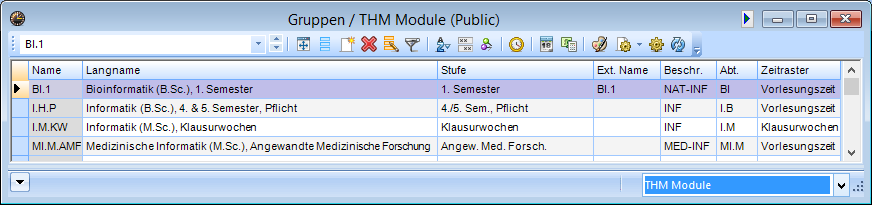
\includegraphics[width=1\textwidth]{Gruppen}
	\vspace{-15pt}
	\caption{Gruppen}
	\label{fig:groups}
\end{figure}

\noindent
{\large Attribute\par}
\vspace{8pt}

\noindent
\texttt{Name}: Beinhaltet Hinweise auf den jeweiligen Studiengang, sowie deren spezifische Untergliederung. Typischerweise mit Punkten getrennt.\\

\noindent
\texttt{Langame}: Der ausgeschriebene Name des Studiengangs mit Abschluss in runden Klammern, gefolgt von Untergliederungsteile, getrennt durch Kommas.\\

\noindent
\texttt{Ext. Name}: (Pflicht bei Fachbereichsübergreifende Gruppen, sonst optional, siehe auch 
\secref{sec:ext-name})\\

\noindent
\texttt{Stufe}: Eine Kurzfassung der Untergliederung. Diese Angabe wird als Name in der Stundenplan-Navigation in THM Organizer benutzt.(Pflicht)\\

\noindent
\texttt{Beschr.} (Fachkompetenz): Assoziiert die Gruppe mit einer Fachkompetenz. (Pflicht. Siehe \secref{subsec:fachkompetenzen}))\\

\noindent
\texttt{Abt.} (Studiengang): Assoziiert die Gruppe und ihre Unterrichte mit einem Studiengang. (Pflicht)\\

\newpage

\noindent
\texttt{Zeitraster}: Assoziiert die Gruppe mit einem Zeitraster. Standardmäßig ist der Wert dieser Spalte ``Hauptzeitraster". Falls Multi-Zeitraster verwendet wird, kann man eingepflegte Zeitraster auswählen. (Pflicht. Wird automatisch mit einem default Wert gefüllt. Siehe auch \nameref{sec:zeitraster})

\subsubsection{Zeitraster \& Klausurwochen}
\label{sec:zeitraster}

Zeitraster legen die Blöcke fest in dem man Unterrichtsinstanzen unterbringen kann. An der THM haben wir bisher zwei feste Zeitraster, eine für Vorlesungen und eine für die Klausurwochen. Solche Zeitraster sind in Untis mit Gruppen assoziiert. Das hat Konsequenzen für unsere Modellierung der Klausurwochen, denn wenn Zeitraster nur mit Gruppen assoziiert werden können, muss es sinnvolle Gruppen geben, um die Klausuren der Klausurwochen zu modellieren.\\
\\
In Fachbereich MNI haben wir eine Klausurwochen-Gruppe pro Studiengang angelegt. Diese verwenden die zweistündige Zeitraster der Klausurwochen. Klausuren können damit Untis-intern recht gut abgebildet werden. Zur Zeit kann Untis die zusätzliche Raster aber nicht exportieren, dass hat als Folge, dass Organizer sie deshalb noch nicht korrekt anzeigen kann.\\

\section{Dozenten}

\begin{wrapfigure}{r}{0.08\textwidth}
	\vspace{-70pt}
	
\includegraphics[width=.08\textwidth]{dozenten-menu}
\end{wrapfigure}

\vspace{25pt}

Dozenten, auch Lehrer in Untis genannt, bezeichnen festangestellte Dozenten, Lehrbeauftragte, Tutoren, Vortragende, Seminarleiter. Kurz gesagt, alle die für eine Veranstaltung oder einen Unterricht verantwortlich sind.\\
\\
Sie erreicht man von der \texttt{Start} Leiste in dem man \texttt{Dozenten} aufklappt und \texttt{Stammdaten} auswählt.\\

\begin{figure}[h]
	\centering
	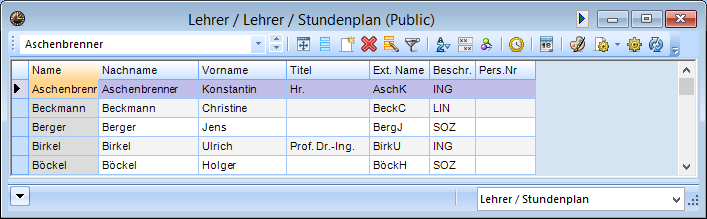
\includegraphics[width=.8\textwidth]{Teachers}
	\vspace{-5pt}
	\caption{Dozenten}
	\label{fig:teachers}
\end{figure}

\noindent
{\large Attribute\par}
\vspace{8pt}

\noindent
\texttt{Name}: Typischerweise wird hier den Nachnamen eingetragen, bei Uneindeutigkeiten können Buchstaben aus den Vornamen und ggf. weitere Nachnamen hinzugefügt.\\

\noindent
\texttt{Nachname}: Die Nachnamen des Dozenten.\\

\noindent
\texttt{Vorname}: Die Vornamen des Dozenten.(Empfohlen)\\

\noindent
\texttt{Ext.Name}: (Pflicht bei Dozenten die in mehreren Fachbereiche tätig sind, sonst Optional, siehe auch 
\secref{sec:ext-name})\\

\noindent
\texttt{Beschr.} (Kompetenz): Assoziiert der Dozent mit einer Fachkompetenz. (Pflicht, siehe   \secref{subsec:fachkompetenzen}))\\

\noindent
\texttt{Pers.Nr} (THM Benutzerkennung): Die THM Benutzerkennung des Dozenten. Erlaubt die eindeutige Zuordnung des Dozenten und ermöglicht ggf. die Verlinkung auf einem Benutzer-Profile aus THM Organizer. (Optional)\\

\section{Räume}

\begin{wrapfigure}{r}{0.08\textwidth}
	\vspace{-80pt}
	
\includegraphics[width=.08\textwidth]{raume-menu}
\end{wrapfigure}

\vspace{35pt}

Räume bezeichnen sämtliche Orte, an denen Unterrichte, Vorträge, Sitzungen und sonstige planungsrelevante Ereignisse stattfinden. Obwohl klassische Veranstaltungsräume, wie Hör- und Seminarräume den Großteil des Raumbestands ausmachen, müssen hier auch außergewöhnliche Örtlichkeiten wie "Grillplatz", "Kongresshalle" oder "Online" aufgeführt sein, damit möglichst ausnahmslos alle Unterrichte mit einem Ort versehen werden können.\\
\\
Von der \texttt{Start} Leiste drückt man klappt man \texttt{Räume} auf und wählt \texttt{Stammdaten} aus.

\begin{figure}[h]
	\centering
	\includegraphics[width=.8\textwidth]{Rooms}
	\vspace{-5pt}
	\caption{Räume}
	\label{fig:rooms}
\end{figure}

\noindent
{\large Attribute\par}
\vspace{8pt}

\noindent
\texttt{Name}: Der Raum Name. Damit die Namen Campus-übergreifend eindeutig sind, wird der Bezeichner für A und C Gebäuden zu ``A10", bzw. ``C10".\\

\noindent
\texttt{Langname}: Die aktuelle Bezeichnung für den Raum.\\

\noindent
\texttt{Ext.Name}: Identisch mit \texttt{Name}. (Pflicht)\\

\noindent
\texttt{Beschr.} (Raumkategorie): Die Kategorie des Raumes. Wird in THM Organizer für Raumplan-Navigation verwendet. (Pflicht, siehe \secref{subsec:room-category})\\

\noindent
\texttt{Kapaz.} (Kapazität): Die Anzahl der Sitzplätze / Rechnerplätze. (Optional)\\

\noindent
\texttt{Statistik} (Ausstattung): Einstellige Bezeichner für die Raumausstattung, wie Overhead (O) oder Beamer (B). Die Bezeichner werden durch Kommata getrennt. Diese werden von Untis eingefügt, der Benutzer braucht nur die Buchstaben einzutragen. (\textbf{Optional})\\

\subsubsection{Raumgruppen}

Raumgruppen sind Gruppierungen von Räumen nach z.B. Typ, Ausstattung, Kapazität, Verwendungszweck, oder eine Kombination daraus. In \figref{fig:roomgroups} sieht man drei der Gruppen der Fachbereich MNI verwendet. Die erst Gruppe, LPC, beinhaltet eine Auflistung der Rechnerlabore in Gebäude A20, jeweils von gleichen Typ, mit einer ähnlichen Ausstattung und Kapazität.\\
\\
Die Verwendung von Raumgruppen ist für die Planung nicht zwingend notwendig, sie eine Planung, die unabhängig von konkreten Räumen ist und nur Raumtypen betrachtet. Das ist in den meisten Fällen genau das was man in der Planung möchte, denn häufig ist der konkret Raum nicht wichtig. Mehr dazu in \chapref{chap:lessons}.\\
\\ 
Von der \texttt{Start} Leiste drückt man klappt man \texttt{Räume} auf und wählt \texttt{Raumgruppen} aus.

\begin{figure}[h]
	\centering
	\includegraphics[width=.8\textwidth]{RoomGroups}
	\vspace{-5pt}
	\caption{Raumgruppen}
	\label{fig:roomgroups}
\end{figure}

\noindent
{\large Attribute\par}
\vspace{8pt}

\noindent
\texttt{Raum}: Eine Komma-getrennte Liste der Räume, die dieser Gruppe gehören. (Pflicht, sofern verwendet)\\

\newpage

\section{Fächer}

\begin{wrapfigure}{r}{0.08\textwidth}
	\vspace{-80pt}
	\includegraphics[width=.08\textwidth]{facher-menu}
\end{wrapfigure}

\vspace{35pt}

Fächer sind die Namensträger für Unterrichte und Unterrichtsinstanzen. Sie geben einen Hinweis darauf, welche Lerninhalte in einem Unterricht oder Unterrichtsinstanz vermittelt werden und sind an der THM (praktisch immer) identisch mit Modulen.\\
\\
Zum Beispiel besteht das Modul ``International Marketing" \hspace{1pt} im Studiengang Unternehmensführung aus mehrere Fächer, im Stundenplan ist nur ein Name für alle solche Fächer gewollt. Im Gegensatz dazu stehen Module wie ``Theorie des Entwerfens I" \hspace{1pt} aus dem Studiengang Bauingenieurwesen, hier sind die Namen der untergeordneten Fächer Einführung ins Entwerfen und Baugeschichte der Ausgabe gewollt und müssen deshalb getrennt eingepflegt werden.\\
\\ 
Fächer haben die besondere Eigenschaft, dass sie nicht in der Periode "Schuljahr" gepflegt werden brauchen, denn jegliche Änderungen an einem Fach sind sofort in allen Perioden sichtbar.\\
\\
Um ein Fach zu erstellen oder zu bearbeiten, muss man in der \texttt{Start} Leiste \texttt{Fächer} aufklappen und \texttt{Stammdaten} auswählen.

\begin{figure}[h]
	\centering
	\includegraphics[width=.8\textwidth]{Subjects}
	\vspace{-5pt}
	\caption{Fächer}
	\label{fig:subjects}
\end{figure}

\noindent
{\large Attribute\par}
\vspace{8pt}

\noindent
\texttt{Text} (Modulnummer): Die Modulnummer des Faches/Moduls. Hier ist entscheidend, wie die Module in LSF abgelegt werden, denn diese Angabe ist notwendig für die automatische Weiterleitung auf Modulbeschreibungen im THM Organizer. Bei Module, die aus mehreren Fächern bestehen, ist es nicht geregelt auf welche Hierarchie-Ebene die Zuordnung zu einer Modulbeschreibung liegt (Modul/Fach). In diesen Fällen sollten wir mit der LSF Verantwörtlichen reden um Klarheit zu beschaffen. (Empfohlen)\\

\noindent
\texttt{Beschr.} (Kompetenz): Assoziiert das Fach mit einer Kompetenz. (Pflicht, siehe \secref{subsec:fachkompetenzen})\\

\section{Verläufe (Unterrichtsgruppen)}
\label{sec:unterrichtsgruppen}

\noindent
Unterrichtsgruppen sind terminliche Begrenzungen von Unterrichten. Dort kann man feste Start- und Enddaten angeben, sowie den Verlauf zwischen diese zwei Daten.\\

\begin{wrapfigure}{r}{0.4\textwidth}
	\vspace{-14pt}
	\centering
	\includegraphics[width=.39\textwidth]{unterrichtsgruppen-symbol}
	\vspace{-5pt}
	\caption{Unterrichtsgruppen im Menü}
\end{wrapfigure}

\noindent
Unterrichtsgruppen findet man in der \texttt{Start} Leiste im Rubrik \texttt{Module}. Es sind bereits in jede Schule Unterrichtsgruppen eingetragen und konfiguriert, diese müssen lediglich den Gegebenheiten der jeweiligen Fachbereiche angepasst werden. Welche Verläufe Ihnen eingerichtet sind und wie deren Lauf gestaltet wird, schlagen Sie am besten im Programm nach.\\

\begin{wrapfigure}{r}{0.4\textwidth}
	\label{fig:unterrichtsgruppen-symbol}
	\centering
	\includegraphics[width=.39\textwidth]{unterrichtsgruppen-ansicht}
	\vspace{-5pt}
	\caption{Unterrichtsgruppen Ansicht}
	\label{fig:unterrichtsgruppen-ansicht}
	\vspace{-115pt}
\end{wrapfigure}

\noindent
{\large Attribute\par}
\vspace{8pt}

\noindent
\texttt{Von}: Das Startdatum der Unterrichtsgruppe. (Pflicht)\\

\noindent
\texttt{Bis}: Das Enddatum der Unterrichtsgruppe. (Pflicht)\\

\vspace{54pt}

\noindent
{\large Kalender\par}
\vspace{8pt}

\begin{wrapfigure}{r}{0.4\textwidth}
	\vspace{-14pt}
	\centering
	\includegraphics[width=.39\textwidth]{unterrichtsgruppen-kalender-ansicht}
	\vspace{-5pt}
	\caption{Unterrichtsgruppen Kalender}
	\label{fig:unterrichtsgruppen-kalender-ansicht}
	\vspace{14pt}
\end{wrapfigure}

\noindent
Unterrichtsgruppen eignen sich sehr gut dafür die Periodizität von Unterrichten sehr fein auf die Wochen abzustimmen - damit können z.B. vorlesungsfreie Zwischenzeiten (wie Weihnachten) berücksichtigt werden. Hierfür verwendet man die Schuljahres-Ansicht. In dieser Ansicht kann man Datenbereiche überstreichen oder einzelne Tage anklicken, um diese in den Verlauf der Unterrichtgruppe zu übernehmen oder zu entfernen. An grünen Tagen werden assoziierte Unterrichte stattfinden können. An weißen Tagen, sowie orangen (Ferien), werden assoziierte Unterrichte nicht stattfinden können. Schließlich klickt man auf \texttt{Ok} oder \texttt{Übernahme}, um die Änderungen geltend zu machen.\\







\chapter{Stundenplanung}
\label{chap:schedules}

\section{Manuelle Stundenplanung}

Für die manuelle Planung wird vorerst nur auf die \texttt{Klassenplan Hoch} oder \texttt{Lehrerplan Hoch}-Ansichten eingegangen, weil von der \texttt{Raumplan Hoch} und \texttt{Fachplan Hoch} darf man nichts planen und letzteres liefert ohnehin nur Unfug.\\
\\
Um zu diesen Ansichten zu gelangen klickt man auf den Pfeil nach Unten unter der jeweilige Ressource, dann auf der entsprechende Menüeintrag.

\subsection{Fensterbereiche}
\label{sec:stundenplan-fensterbereiche}

Die Fensterbereiche wurden im allgemeinen im \secref{sec:fensterbereiche}, kurz erläutert. Weil viele wichtige Informationen verteilt über das gesamte Fenster angezeigt werden, wird hier nochmal darauf eingegangen.\\
\\
Der Rasterbereich in Stundenplan-Ansichten ist sowohl für die Darstellung als auch die Gestaltung der Pläne verantwortlich und teilt sich in einen Datum-Bereich, einen Stundenplan-Bereich und einen Bereich für nicht verplante Stunden auf. Im Infobereich stehen Informationen zu der markierte/aktive Block. Sollten Sie noch keinen angeklickt haben, wählt Untis den ersten Block im Stundenplan-Bereich aus.\\
\\
Als Beispiel wird in \figref{fig:klassenplan-hoch-ansicht} ein sehr gefüllter Plan von Fachbereich KMUB dargestellt.

\newpage

\begin{figure}[h]
	\centering
	\includegraphics[width=.8\textwidth]{klassenplan-hoch-ansicht}
	\vspace{-5pt}
	\caption{Klassenplan-Hoch-Ansicht}
	\label{fig:klassenplan-hoch-ansicht}
\end{figure}

\subsubsection{Datumbereich}

\begin{wrapfigure}{r}{0.4\textwidth}
	\centering
	\vspace{-14pt}
	\includegraphics[width=.38\textwidth]{zeitbereich}
	\vspace{-5pt}
	\caption{Zeitbereich Auswahl}
	\label{fig:zeitbereich}
	\vspace{14pt}
	\includegraphics[width=.38\textwidth]{woche}
	\vspace{-5pt}
	\caption{Woche Auswahl}
	\label{fig:woche}
\end{wrapfigure}

Das Datum-Bereich zeigt an für welchen Daten der angezeigte Plan gilt. Man kann zwischen einer Perioden-Darstellung und einer Wochen-Darstellung in dem man das Kalender-Symbol anklickt und den entsprechenden Eintrag auswählt. In \figref{fig:klassenplan-hoch-ansicht}, gilt der angezeigte Plan für das gesamte Wintersemester.\\
\\
Sollte man den Wochen-Ansicht ausgewählt haben werden die Anfangs- und Enddatum der Woche hier dargestellt. Zwischen den beiden Daten gibt es zwei Knöpfe: \UParrow \hspace{2pt} und \DOWNarrow. In dem man auf diese drückt kann man Wochenweise in der Rückwärts \UParrow \hspace{2pt} oder Vorwärts \DOWNarrow \hspace{2pt} durch die Wochen des Schuljahres blättern. In der editierbaren Feld in dem das Startdatum sich befindet kann man auch auf dem $\vee$ klicken um ein Kalender zu öffnen. Mit diesem kann man ggf. Monats- oder gar Jahresweise blättern. Obwohl man die Zahlen des Startdatums bearbeiten kann bewirkt die Änderung diese Angaben nichts.

\subsubsection{Stundenplan-Bereich}

Der Stundenplan-Bereich zeigt die geplanten Stunden abhängig von der ausgewählte Ressource an. Der aktive Block wird mit einer rot \& gelb gefärbten Umrandung angezeigt. Sollte der aktive Block Unterrichte beinhalten werden die andere Stunden dieser mit einem einer blau \& gelb gefärbte Umrandung ebenfalls hervorgehoben.\\

\begin{wrapfigure}{r}{0.3\textwidth}
	\centering
	\includegraphics[width=.29\textwidth]{getrennte-unterrichte}
	\vspace{-5pt}
	\caption{Getrennte Darstellung einer Unterrichtsstunde}
	\label{fig:getrennte-unterrichte}
\end{wrapfigure}

\noindent
Die Informationen die Angezeigt werden in der jeweilige Raster Block sind fast beliebig einstellbar und man kann diese Einstellungen speichern damit alles immer so aussieht wie man es braucht. Man sollte unbedingt eine Ansicht speichern in dem alle Unterrichte einer Stunde getrennt angezeigt werden. \figref{fig:getrennte-unterrichte} zeigt ein solche Darstellung der gleichen aktiven Unterrichtsstunde wie in \figref{fig:klassenplan-hoch-ansicht}. Dies ermöglicht die Unterrichte einzeln anzusprechen für Raumzuweisungen, oder um sie zu einem späteren Zeitpunkt einzelnen umplanen zu dürfen. Wenn Stunden so dargestellt werden wie in \figref{fig:klassenplan-hoch-ansicht}, um einen einzelnen Unterricht umplanen zu können, müssten alle vier aus dem Plan gezogen werden und neu verplant werden.\\
\\
Sofern man die Darstellung in Untis nach außen Präsentieren möchte, empfiehlt es sich zwei Stundenplan-Formate zu speichern, wo die zweite nur für die Außendarstellung gedacht ist. Für diesen Zweck ist auch der Plan \figref{fig:klassenplan-hoch-ansicht} gedacht. Es zeigt ein Vielzahl an Informationen ohne durch die Trennung der Unterrichte aufgeteilt zu werden. Mehr dazu \secref{sec:stundenplan-einstellungen}.

\subsubsection{Nicht verplante Stunden}

Im Bereich rechts vom Stundenplan stehen die nicht geplanten Stunden. Bis drei werden die Anzahl an nicht verplanten Stunden eines Unterrichts als Kästchen direkt angezeigt, ab vier wird der Zahl in einem Oval an der obere Kante der Stunden dargestellt.\\
\\
Sollten viele Unterrichte einer Ressource noch nicht verplant sein, kann in diesem Bereich ein ziemliches Durcheinander herrschen. Unter Anderem, können einige Unterrichte soweit nach rechts verschoben sein, dass sie nicht mehr angezeigt werden. Sollte dies der Fall sein, können Sie die angezeigte Unterrichte/Stunden neu gruppieren lassen. Hierzu macht man ein Rechts-Klick irgendwo in diesem Bereich. Ein Kontextmenü erscheint in dem \texttt{N. vpl. Stunden neu gruppieren} als zweite Option erscheint, wählen Sie dieser.

\subsection{Planung}
\label{sec:manuelle-planung}

Die manuelle Stundenplanung geschieht mittels ``Drag \& Drop" Funktionalität. Diese wird anhand \figref{fig:stundenplan-stundenplanung} verdeutlicht. Man zieht dazu eine nicht verplante Stunde von der rechte Seite in einem Block im Stundenplan.\\

\begin{figure}[h]
	\centering
	\includegraphics[width=.8\textwidth]{stundenplan-stundenplanung}
	\vspace{-5pt}
	\caption{Manuelle Stundenplanung}
	\label{fig:stundenplan-stundenplanung}
\end{figure}

\noindent
Planungen für die aktuelle Ressource sieht man schon bevor das Ziehen in grau Dargestellt. Sobald man ein solche Stunde über den Stundenplan-Bereich zieht, passen sich die Farben der 'leeren' Stunden die assoziierte Ressourcen dieser Unterrichtsstunde an.\\
\\
Die aktuelle Position der gezogene Stunde wird mit seiner Umrandung und Inhalt angezeigt und der Block, über den er gerade gezogen wird, bekommt ein mittel Rosa Hintergrund-Farbe, wie in \figref{fig:stundenplan-stundenplanung}, Freitag in der 4. Stunde, zu sehen ist. Zusätzlich, sollte ein Ressourcenkonflikt geben in der Stunde, werden konfliktierende Unterrichte im Infobereich eingeblendet. Im \figref{fig:stundenplan-stundenplanung} würde es ein Konflikt wegen Herr Subke, zwischen den zu planenden Block und der Stunde über den sich er gerade gezogen wird, geben.\\
\\
Leere Stunden in dem es Konflikte geben würde werden standardmäßig violett oder weiß gefärbt. Violett entspricht einen Raumkonflikt, wohingegen weiß ein Dozenten- oder Gruppenkonflikt. In \figref{fig:stundenplan-stundenplanung} werden Montag 3. Block und Dienstag 6. violett dargestellt, denn der gewünschte, sprich im Lehrplan enthaltene, Raum (C.8.01) bereits durch andere Veranstaltungen reserviert worden ist. Mittwochs 1. Stunde und Freitags 4. wären weiß dargestellt, denn in die zwei Blöcke ist Herr Subke anderweitig beschäftigt.\\
\\
Stunden die frei sind werden entweder in ein sehr helles rosa oder ein grün Ton dargestellt. Hell rosa ist der normal Zustand einer freien Stunde, grün Töne sind Empfehlungen des Programmes. Im \figref{fig:stundenplan-stundenplanung} sind 8 Stunden noch Konflikt-frei planbar Samstag 3. Stunde wird empfohlen weil es direkt hinter ein geplanter Block liegt und Samstag hat bisher die wenigsten geplanten Stunden.

\subsection{Entplanung}
\label{sec:manuelle-entplanung}

Wenn man die manuelle Planung verstanden hat, ist die Entplanung großteils intuitiv. In fast allen Fällen zieht man einfach die Stunde vom Plan zur rechten Seite. Bei Unterrichte, die mit Wochenstunden versehen sind, ist es auch damit erledigt. Bei Unterrichte die mit Jahresstunden versehen sind ist die Lage etwas kniffliger.\\
\\
Wenn man eine Stunde, die mit Jahresstunden versehen ist, aus dem Stundenplan-Raster zieht, ist nur diese eine Stunde entplant worden. Sollte man mehrere Stunden entplanen wollen gibt es zwei Möglichkeiten. Hat man die Ansicht so eingestellt, dass Unterrichte im Plan im Fall einer Kollision getrennt dargestellt werden und alle zusammenhängende Unterrichtsstunden als eine Einheit dargestellt werden, kann man diese zusammenhängende Unterrichtsstunden auf einmal vom Stundenplan ziehen. Man kann auch die Anzahl der Stunden reduzieren oder auf null setzen. Bei einer Reduzierung der Stunden werden, zeitlich gesehen, Stunden von hinten nach vorne entplant, d.h. Stunden die später im Schuljahr stattfinden werden eher entplant. Bspw. wenn Unterrichtsstunden in die zweite und dritte Januar Woche, sowie in der erste Woche April, werden erst die Unterrichtsstunden in April entplant, dann die Stunden in der dritte Januar Woche, dann im zweiten. Bei einer Reduzierung auf null, werden entsprechend alle Unterrichtsstunden entplant.\\
\\
Was, die Entplanung von sporadische Unterrichtsstunden verkompliziert, ist, dass Untis davon ausgeht, dass man manuell entplante Stunden noch in der selben Woche stattfinden lassen möchte. D.h. die entplante Stunde ist normalerweise an der Woche in der sie entplant war gebunden. Man kann diese Wochenverbindung umgehen in dem man die \texttt{STRG}-Taste hält bevor man die Stunde oder Stunden aus dem Raster zieht.

\section{Planungsdialog}

Diese Sektion wird als letztes gepflegt.

\section{Automatisierte/Optimierte Planung}

Diese Planungsmöglichkeit werde ich im Frühling angehen.

\section{Übersichtspläne}

Übersichtspläne sind Stundenpläne, die mehrere Ressourcen anzeigen. Obwohl es sie theoretisch in vier Ausrichtungen gibt, siehe \secref{sec:stundenplan-formate}, werden standardmäßig nur zwei Stück in der Menüführung vertreten: \texttt{hoch} (\texttt{30}) und \texttt{quer} (\texttt{20}). Bei Übersichtspläne-\texttt{hoch} werden die ausgewählte Ressourcen als Spalten dargestellt und die Wochenstunden als Zeilen. Übersichtspläne-\texttt{quer} hat entsprechend die Darstellung der Ressourcen (Zeilen) und Wochenstunden (Spalten) vertauscht.\\
\\
Sie würden dank die neuen Auswahlboxen deutlich verbessert, denn man kann jetzt die Ressourcen auswählen die man gerne sehen möchte. Obwohl die Übersichtspläne über die Menüführung von Gruppen, Dozenten und Räume angeboten werden, sind sie in der Umsetzung beliebig kombinierbar, denn \textbf{alle} Ressourcen sind in der Auswahlbox und können mit \texttt{STRG $+$ Klick} einzeln selektiert werden. Als Beispiel habe ich ein Übersichtsplan-\texttt{quer} erstellt mit der Belegungen der großen Räume, wie im \figref{fig:ubersicht-raume-gross} zu sehen.\\
\\
Abgesehen von dem Inhalt der Pläne selbst weichen Übersichtsplan-Fenster nur von Einzelplan-Fenster, siehe \secref{sec:stundenplan-fensterbereiche}, in der Ausrichtung der nicht verplante Stunden. Welche hier unter der Stundenplan-Bereich dargestellt werden.\\
\\
Da die nicht verplante Stunden dargestellt werden kann man theoretisch auch von Übersichtspläne die manuelle Planung durchführen. Allerdings wegen der Ausrichtung und der Anzahl an darzustellende Informationen ist es nicht empfohlen dies zu tun.

\newpage

\begin{figure}[h]
	\centering
	\includegraphics[width=.8\textwidth]{ubersicht-raume-gross}
	\vspace{-5pt}
	\caption{Übersichtsplan große Räume}
	\label{fig:ubersicht-raume-gross}
\end{figure}

Die Anleitung für den Drück wird später ergänzt.













\chapter{Fortgeschrittene Einstellungen}
\label{chap:advanced-settings}

\section{Schaltfläche Personalisierung}
\label{sec:advanced-quick-access}

\begin{appendices}
\chapter{Zusatzmaterial}

\section{Deniffel'sche Raumkategorien}
\label{sec:dennifel}
\begin{multicols}{2}
	\begin{description}
		\item[A1] Seminarraum, 1-20 Plätze
		\item[A2] Seminarraum, 21-33 Plätze
		\item[A3] Seminarraum, 34-47 Plätze
		\item[A4]	Hörsaal,  48- 69 Plätze
		\item[A5]	Hörsaal,  70- 84 Plätze
		\item[A6]	Hörsaal,  85-105 Plätze
		\item[A7]	Hörsaal, 100-150 Plätze
		\item[A8]	Hörsaal, 150-200 Plätze
		\item[A9]	Hörsaal, 200-300 Plätze
		\item[AZ]	Hörsaal, 300-400 Plätze
		\item[B1]	Fachsaal, Physik-Hörsaal (gr.)
		\item[B2]	Fachsaal, Physik-Hörsaal (kl.)
		\item[B3]	Fachsaal, Chemie	Raum	R
		\item[C1]	Fachsaal, Praktikumsraum \\mit. spez. Einbauten
		\item[C2]	Fachsaal, Praktikumsraum \\keine spez. Einbauten
		\item[C3]	Fachsaal, Forschungslabor
		\item[C4]	Fachsaal, Mess-Stand
		\item[C5]	Fachsaal, Nebenlabor
		\item[C6]	Fachsaal, Vorbereitungsraum
		\item[C9]	Fachsaal, Betriebsraum
		\item[D1]	Rechnerraum, allgemein
		\item[D2]	Rechnerraum, fachspez.
		\item[D3]	Rechnerraum, fachspez. (Forschung)
		\item[D4]	Rechnerraum, Peripherie- / Geräteraum
		\item[D5]	Rechnerraum, Serverraum
		\item[D7]	Rechnerraum, Schulung
		\item[F1]	Projektraum, allgemein
		\item[F2]	Projektraum, Gruppenarbeitsraum
		\item[F3]	Projektraum, Übungen
		\item[F5]	Projektraum, Studiebüro
		\item[F6]	Projektraum, Sozialraum
		\item[H1]	Sonstige Räume, Archiv
		\item[H2]	Sonstige Räume, Seminar-Nebenraum
		\item[H3]	Sonstige Räume, sonstiges Lager
		\item[H4]	Sonstige Räume, Labor Lager
		\item[H5]	Sonstige Räume, Abstellraum
		\item[I1]	Büro, Büro	Raum
		\item[I2]	Büro, Labor-Ingenieur
		\item[I3]	Büro, Werkstatt
		\item[I4]	Büro, Besprechungen
		\item[I5]	Büro, Ergänzungsraum
		\item[I6]	Büro, Videokonferenzen
		\item[UNIMA]	Raum, Uni Marburg
		\item[W1]	Werkstatt, Feinmechanik
		\item[W2]	Werkstatt, Metall
		\item[W5]	Werkstatt, Elektronik
		\item[W7]	Werkstatt, Nebenraum
		\item[W9]	Werkstatt, Lager
		\item[X]	Raum, nicht bekannt
	\end{description}
\end{multicols}

\section{Unterrichtsgruppen MNI 2014/2015}
\label{sec:unterrichtsgruppen-values}
\begin{description}
	\item[WS.E]	Einführungswoche - WS 06.10.2014 - 11.10.2014	 	 	 	
	\item[WS]	Wintersemester	13.10.2014 - 31.01.2015	
	\item[WS.A]	Wintersemester (Woche A) 13.10.2014 - 31.01.2015
		\begin{itemize}
			\item 13.10.2014 - 18.20.2014
			\item 27.10.2014 - 01.11.2014
			\item 10.11.2014 - 15.11.2014
			\item 24.11.2014 - 29.11.2014
			\item 08.12.2014 - 13.12.2014
			\item 12.01.2015 - 17.01.2015
			\item 26.01.2015 - 31.01.2015
		\end{itemize}
	\item[WS.B]	Wintersemester (Woche B) 20.10.2014 - 24.01.2015
		\begin{itemize}
			\item 20.10.2014 - 25.10.2014
			\item 03.11.2014 - 08.11.2014
			\item 17.11.2014 - 22.11.2014
			\item 01.12.2014 - 06.12.2014
			\item 15.12.2014 - 20.12.2014
			\item 19.01.2015 - 24.01.2015
		\end{itemize}
	\item[WS.P]	Projektwoche - WS 05.01.2015 - 10.01.2015	 	 	 	
	\item[WS.K1] Klausurwoche 1 - WS	2/2/2015	2/8/2015	 	 	 	
	\item[WS.K2] Klausurwoche 2 - WS	2/9/2015	2/15/2015	 	 	 	
	\item[WS.B1] Blockveranstaltungen 1 - WS	2/16/2015	3/1/2015	 	 	 	
	\item[WS.B2] Blockveranstaltungen 2 - WS	3/2/2015	3/15/2015	 	 	 	
	\item[WS.K3] Klausurwoche 3 - WS	3/23/2015	3/29/2015	 	 	 	
	\item[WS.K4] Klausurwoche 4 - WS	3/30/2015	4/5/2015	 	 	 	
	\item[SS.E]	Einführungswoche - SS	4/6/2015	4/12/2015	 	 	 	
	\item[SS] Sommersemester	4/13/2015	7/19/2015  6/1	6/7
	\item[SS.A] Sommersemester (Woche A)	4/13/2015	7/19/2015 4/20	4/26
		SS.A	Sommersemester (Woche A)	4/13/2015	7/19/2015 5/4	5/10
		SS.A	Sommersemester (Woche A)	4/13/2015	7/19/2015 5/18	5/24
		SS.A	Sommersemester (Woche A)	4/13/2015	7/19/2015 6/1	6/14
		SS.A	Sommersemester (Woche A)	4/13/2015	7/19/2015 6/22	6/28
		SS.A	Sommersemester (Woche A)	4/13/2015	7/19/2015 7/6	7/12
	\item[SS.B]	Sommersemester (Woche B)	4/20/2015	7/12/2015 4/27	5/3
		SS.B	Sommersemester (Woche B)	4/20/2015	7/12/2015 5/11	5/17
		SS.B	Sommersemester (Woche B)	4/20/2015	7/12/2015 5/25	6/7
		SS.B	Sommersemester (Woche B)	4/20/2015	7/12/2015 6/15	6/21
		SS.B	Sommersemester (Woche B)	4/20/2015	7/12/2015 6/29	7/5
	\item[SS.P]	Projektwoche - SS	6/1/2015	6/7/2015	 	 	 	
	\item[SS.K1]	Klausurwoche 1 - SS	7/20/2015	7/26/2015	 	 	 	
	\item[SS.K2]	Klausurwoche 2 - SS	7/27/2015	8/2/2015	 	 	 	
	\item[SS.B1]	Blockveranstaltungen 1 - SS	8/3/2015	8/16/2015
	\item[SS.B2]	Blockveranstaltungen 2 - SS	8/17/2015	8/30/2015
	\item[SS.K3]	Klausurwoche 3 - SS	9/21/2015	9/27/2015	 	 	 	
	\item[SS.B3]	Blockveranstaltungen 3 - SS	9/7/2015	9/20/2015
	\item[SS.K4]	Klausurwoche 4 - SS	9/28/2015	10/4/2015 	 	 	
		
\end{description}
	
\end{appendices}

\end{document}          
